A convolutional Neural Network (CNN) is a specialized kind of neural networks employs a mathematical operation called convolution.
Convolution is a mathematical operation that combines two functions to produce a real valued output. In the context of CNNs, it is used to extract features hierarchically from input data,
such as images, followed by non-linear activation functions to introduce non-linearity into the model. After extracting features through convolutional layers and pooling layers, the output is passed through fully connected layers to perform classification or regression tasks.
The convolution operation can be mathematically expressed as follows:
\begin{equation}
 z{(t)} = (x*w)\cdot(t)
 \label{eq:convolutionbasic}
\end{equation}
where $z(t)$ is the output signal, $x$ is the input image, $w$ is the kernel (or filter), and $t$ represents the spatial location in the output feature map. The convolution operation involves sliding the kernel across the input signal and computing the dot product at each position to produce the output feature map.
\subsubsection{Forward Pass and Activation Functions}
\begin{equation}
 z^{(l)}_{i,j} = (W*X)\cdot(i,j)=\sum_{m} \sum_{n} W^{(l)}_{m,n} \cdot x_{(i+m, j+n)}
 \label{eq:convolution}
\end{equation}
where $z^{(l)}_{i,j}$ is the pre-activation value at position $(i,j)$ in layer $l$, $W$ is the weight matrix (or filter), $X$ is the input image, and $(i,j)$ represents the spatial location in the feature map.
The kernel $W$ is a small matrix of weights that is sliding across the input image $X$ to capture the local features. The output feature map $z^{(l)}_{i,j}$ is generated by summing the element-wise product of the kernel and the corresponding region of the input image.
This operation allows CNNs to learn spatial hierarchies of features.

In a CNN, the forward pass is the sequential convolution operation of an input image  trough series of layers to produce predicted output.
At each layer $l$, the feature map is computed applying the convolution operation defined in Equation \ref{eq:convolution} followed by the non-linear activation function $\phi(\cdot)$. The mathematical representation of the forward pass can be expressed as follows:
\begin{equation}
    a^{(l)} = \phi(z^{(l)})
    \label{eq:activation}
\end{equation}
where $a^{(l)}$ is the activated output layer $l$, $z^{(l)}$ is the output of the convolution operation at layer $l$,
and $\phi(\cdot)$ is the activation function. 

Convolutional Neural Networks can utilize various activation functions to express non-linearity, such as sigmoid, tanh, and Rectified Linear Unit (ReLU), which can be mathematically defined as follows:
\begin{equation}
    \sigma(z)=\frac{1}{1+e^{-z}}
    \label{eq:sigmoidfunc}
\end{equation}
Sigmoid activation function, as shown in Equation \ref{eq:sigmoidfunc} maps the input to a real value between (0,1) which is useful for binary classification problems. Even though sigmoid function is widely used,
it suffers from vanishing gradient problem , which can hinder the training of deep neural networks. The vanishing gradient problem occurs when the gradient becomes almost zero for large or small values of $z$.
The graph of the sigmoid function is shown in Figure \ref{fig:sigmoid}
\begin{figure}[ht]
    \centering
    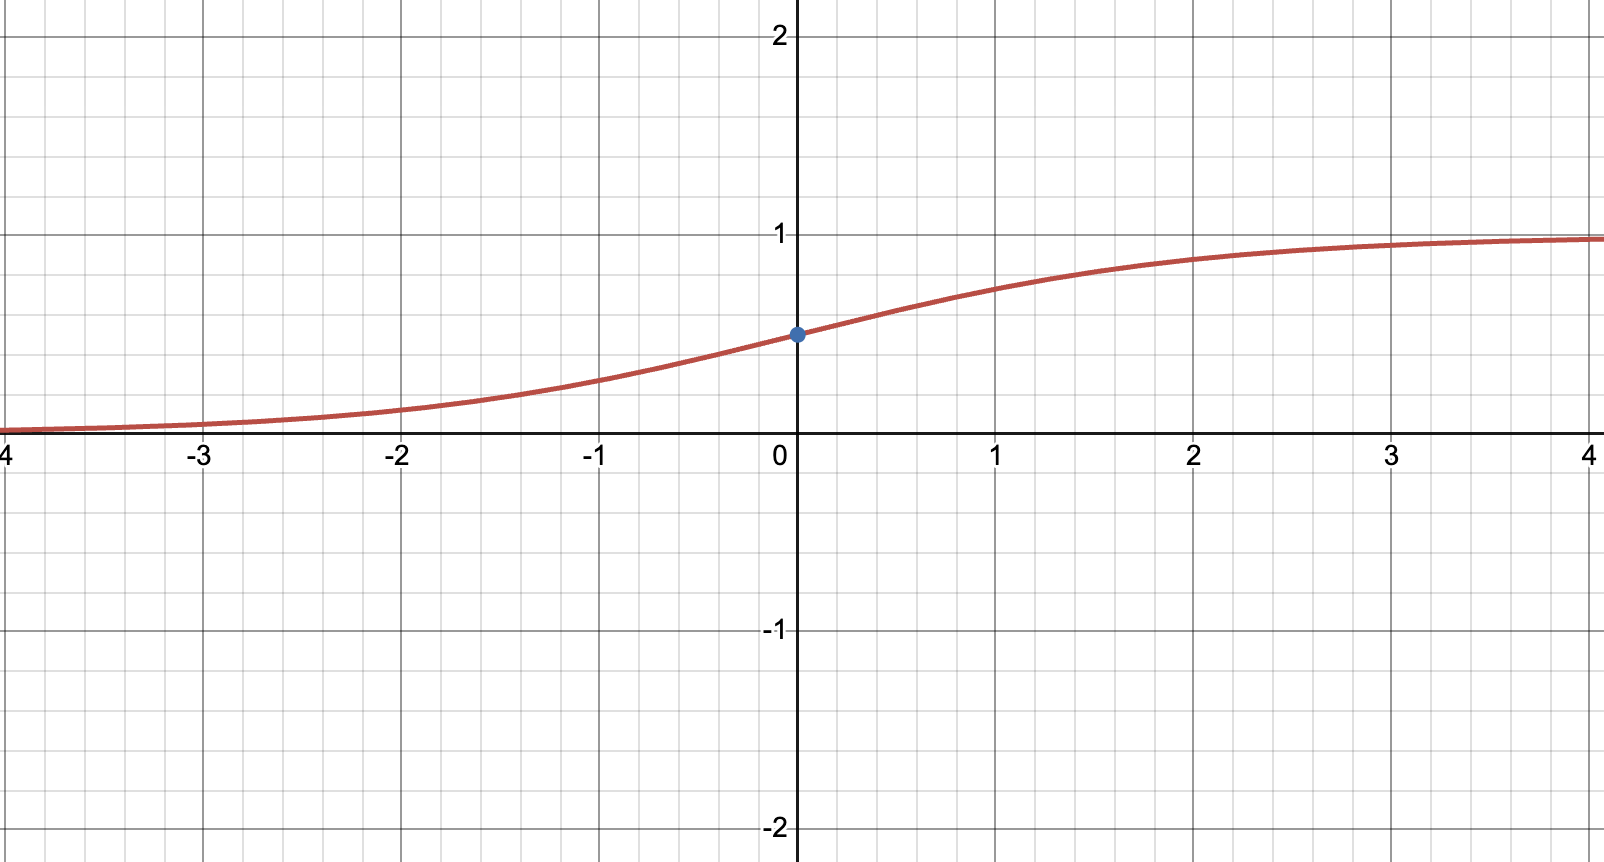
\includegraphics[width=0.5\textwidth]{figures/sigmoid.png}
    \caption{Graphical representation of the sigmoid activation function.}
    \label{fig:sigmoid}
\end{figure}
\begin{equation}
    \tanh(z)=\frac{e^z-e^{-z}}{e^z+e^{-z}}
    \label{eq:tanhfunc}
\end{equation}
Tanh activation function, as shown in Equation \ref{eq:tanhfunc} maps the input values to a range of (-1,1) which can be useful for certain classification tasks where the output can be negative.
However, similar to sigmoid function, tanh also suffers from the vanishing gradient problems. The graph of the tanh function is shown in Figure \ref{fig:tanh}
\begin{figure}[ht]
    \centering
    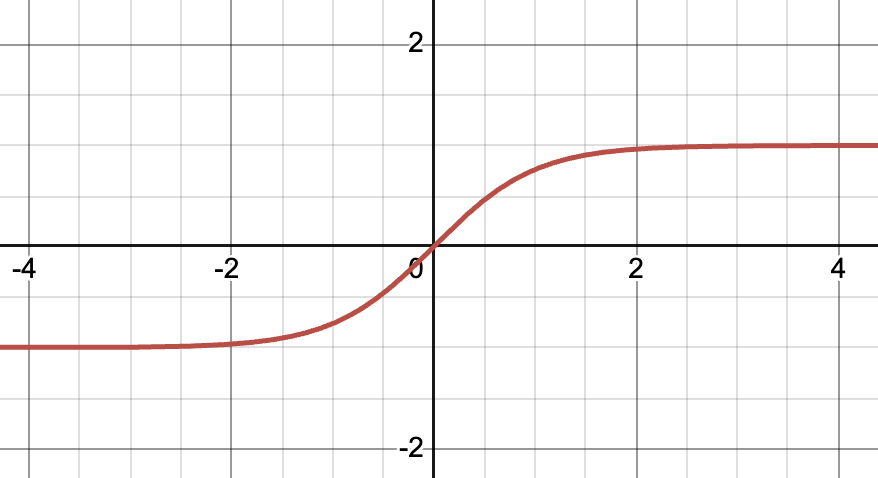
\includegraphics[width=0.5\textwidth]{figures/tanh.png}
    \caption{Graphical representation of the tanh activation function.}
    \label{fig:tanh}
\end{figure}
ReLU introduces non-linearity by mapping input values smaller than zero to zero and keeping positivive values unchanged. The mathematical representation of the ReLU function is given by Equation \ref{eq:relufunc}. 
\begin{equation}
    \text{ReLU}(z) = \max(0, z)
    \label{eq:relufunc}
\end{equation}
ReLU is computationally efficient and helps mitigate the vanishing gradient problem, compared to sigmoid and tanh functions. The function converges faster during training and allows for deeper networks, which is the reason why it is widely used in CNNs. However, the ReLU function can suffer from the "Dying ReLU" problem, which occurs when the input values are negative and the gradient becomes zero. In that case, the neurons will be regarded as inactivated or dead.  The graph of the ReLU function is shown in Figure \ref{fig:relu}
\begin{figure}[ht]
    \centering
    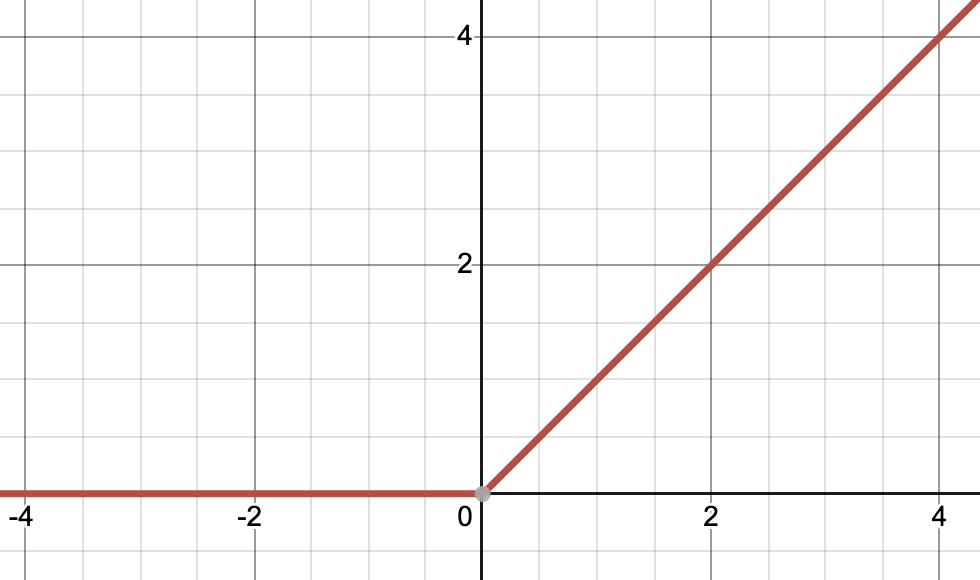
\includegraphics[width=0.5\textwidth]{figures/relu.png}
    \caption{Graphical representation of the ReLU activation function.}
    \label{fig:relu}
\end{figure}

For the output layer, the Softmax function maps the  
raw output scores of the final layer to class probabilities:

\begin{equation}
\hat{y}_k = \frac{e^{z_k}}{\sum_{j} e^{z_j}}
\label{eq:softmax}
\end{equation}

Where $\hat{y}_k $ denotes the predicted probability corresponding to class $k$.
${z_k}$ denotes the raw output score for class $k$ from the final layer of the network, and the denominator sums over all classes iterating $j$ to compute the normalization factor. The softmax function ensures that the output probabilities sum to 1, making it suitable for multi-class classification problems. 

\subsubsection{Loss Function and Optimization}

Given a training set Given a training set $\mathcal{D} = \{(x_i, y_i)\}_{i=1}^n$, 
where $x_i$ denotes the $i$-th input image and $y_i$ the actual output of the model, the model is trained by minimizing the empirical risk using a loss function
that quantifies the distance between the predicted value and the actual value :

\begin{equation}
\mathcal{L}(\theta) = \frac{1}{n} \sum_{i=1}^{n} 
\ell(f_\theta(x_i), y_i)
\label{eq:empiricalrisk}
\end{equation}

Where $\theta$ denotes the model parameters, $f_\theta(x_i)$ 
is the predicted output, $n$ denotes the number of samples and $\ell(\cdot, \cdot)$ is the loss 
function corresponding to the task. Especially for classification tasks, cross-entropy loss often referred to as the softmax loss is commonly used to measure the probability distribution
difference between obtained and actual output. \cite{Li2020ASO} In multiple class datasets, such as CIFAR-10, MNSIT, ImageNet the cross-entropy loss is defined as:

\begin{equation}
\ell(\hat{y}, y) = -\sum_{k=1}^{K} y_k \log \hat{y}_k
\label{eq:crossentropy}
\end{equation}

Where $K$ is the number of classes, $y_k \in \{0,1\}$ is the 
ground-truth indicator for class $k$, and $\hat{y}_k$ is the 
predicted probability defined in Equation \ref{eq:softmax}. 
The training objective is therefore to find the optimal 
parameters:

\begin{equation}
\theta^* = \arg\min_{\theta} \mathcal{L}(\theta)
\label{eq:optimization}
\end{equation}

\subsubsection{Backpropagation and Gradient Descent}

To minimize the loss function defined in Equation \ref{eq:empiricalrisk}, 
the model parameters are updated iteratively using gradient 
descent algorithms. The gradient descent algorithm can be expressed as follows:
\begin{equation}
\theta_{t+1} = \theta_t - \eta \nabla_\theta \mathcal{L}(\theta_t)
\label{eq:gradientdescent}
\end{equation}

Where $\theta_{t+1}$ denotes the updated parameters at iteration $t+1$, $\theta_t$ denotes the previous parameters at iteration $t$, $\eta$ is the learning rate, and $\nabla_\theta \mathcal{L}(\theta_t)$ is the gradient of the loss function with respect to the parameters at iteration $t$.


In Convolutional Neural Networks (CNNs), the gradients are computed via backpropagation, which 
applies the chain rule to calculate the gradients of the loss 
function. For a layer $l$,the gradient of the loss function 
with respect to the weights is:

\begin{equation}
\frac{\partial \mathcal{L}}{\partial W^{(l)}} = 
\frac{\partial \mathcal{L}}{\partial z^{(l)}} \cdot 
\frac{\partial z^{(l)}}{\partial W^{(l)}}
\label{eq:chainrule}
\end{equation}
Where $\frac{\partial \mathcal{L}}{\partial z^{(l)}}$ denotes the error of the current layer $l$, 
$\frac{\partial z^{(l)}}{\partial W^{(l)}}$ is the input according to the weights of the current layer.
The error signal is propagated backward through the network, allowing for the computation of gradients for each layer.

The simplest gradient descent algorithm is Stochastic Gradient Descent 
\begin{equation}
\theta_{t+1} = \theta_t - \eta \nabla_\theta 
\mathcal{L}_{\mathcal{B}}(\theta_t)
\label{eq:sgd}
\end{equation}

Where $\eta$ is the learning rate. While SGD is effective, 
it applies a uniform learning rate to all parameters. Adam 
extends SGD by maintaining adaptive moment estimates of the 
gradients:

\begin{equation}
m_t = \beta_1 m_{t-1} + (1-\beta_1)\nabla\mathcal{L}, 
\quad v_t = \beta_2 v_{t-1} + 
(1-\beta_2)(\nabla\mathcal{L})^2
\label{eq:adammoments}
\end{equation}

\begin{equation}
\theta_{t+1} = \theta_t - \frac{\eta}{\sqrt{\hat{v}_t} 
+ \epsilon} \hat{m}_t
\label{eq:adamupdate}
\end{equation}

Where $\hat{m}_t = \frac{m_t}{1-\beta_1^t}$ and 
$\hat{v}_t = \frac{v_t}{1-\beta_2^t}$ are bias-corrected 
estimates, $\beta_1$ and $\beta_2$ are decay rates, and 
$\epsilon$ is a small constant for numerical stability. 
Notably, the simplicity bias of SGD-based optimizers toward 
simpler solutions has been identified as a key factor in 
the emergence of spurious correlations and memorization 
during training \cite{yang_yu_4720d432}, which is further 
examined in Section 3.2. 